This is the last comparison between the methods presented in this project. In this section, metaheuristics presented in chapter \ref{chapter:metaheuristics} are compared: the VNS, the Tabu Search, and the Genetic algorithms.

To compare them, larger instances than the previous ones are created. A set of 20 instances with 2000 nodes is randomly built and then they are tested with a time limit of 30 minutes. The results are visible in figure \ref{fig:result-meta}.

\begin{figure}[h]
	\centering
	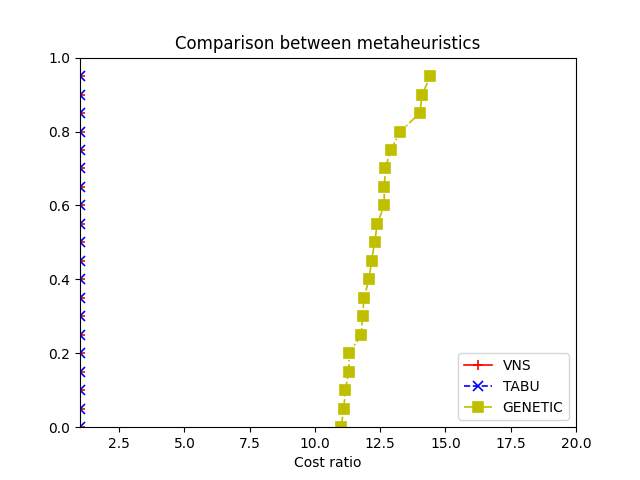
\includegraphics[width=0.6\textwidth]{images/final_meta.png}
	\caption{The comparison between the Matheuristics.}
	\label{fig:result-meta}
\end{figure}

It is possible to notice that genetic algorithms lead to worst solutions. This is due to the fact that the starting population is totally randomly generated and so, within a small time limit, it is difficult to improve as much as in VNS or Tabu Search.

To see the winner of this section it is necessary to zoom the left side of the chart. 

\begin{figure}[h]
	\centering
	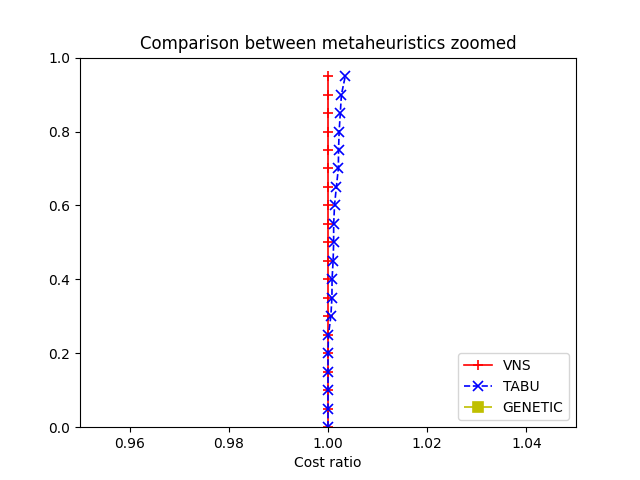
\includegraphics[width=0.6\textwidth]{images/final_meta_zoom.png}
	\caption{The comparison between the Matheuristics.}
	\label{fig:result-meta-zoom}
\end{figure}

In figure \ref{fig:result-meta-zoom} it is evident that the winner of this comparison is the VNS.